\documentclass[10pt,a4paper]{article}
\usepackage[utf8]{inputenc}
\usepackage{amsmath}
\usepackage{amsfonts}
\usepackage{amssymb}
\usepackage{graphicx}
\author{Brock Ellefson}
\title{CSCI468 Problem Set 2}
\begin{document}
\section{For the following sub-problems, consider the following context-free grammer}
\subsection{What are the terminals and non-terminals of this language}
The terminals of this language are: $V_{t} = (x , y)$ \\
The non-terminals of this language are: $V_{n} = (S, A, B)$

\subsection{Describe the strings are generated by this language. Is this a regular language?}
This language is a regular language.

\subsection{Show the derivation of the string $xyxxy\$$ starting from $S$}
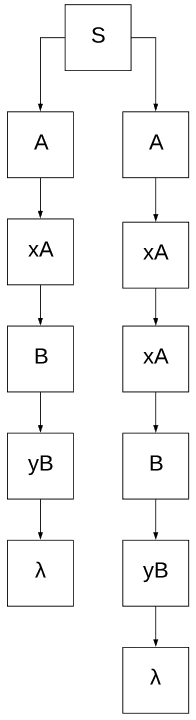
\includegraphics[scale=.5]{parsetree.png}



\end{document}